We now instead imagine the geometry fixed, with the incoming wave $\phi_0$ interacting with the geometry.
The diffraction potential is described by
\[
    \Phi_{\mathrm{D}}(\xvec; t) = \Re{\big( A \phi_{\mathrm{D}} e^{i\omega t} \big)},
\]
where $\phi_{\mathrm{D}} = \phi_0 + \phi_7$.
We may find $\phi_7$ by solving the integral equation
\[
    -\pi \phi_{\mathrm{D}}(\bzhe) + \int_{S_{\mathrm{B}}} \phi_{\mathrm{D}} \partial_{\nhat} \green \,\dee S = -2\pi \phi_0(\bzhe).
\]
\begin{Figure}
    \centering
    \captionsetup{type = figure}
    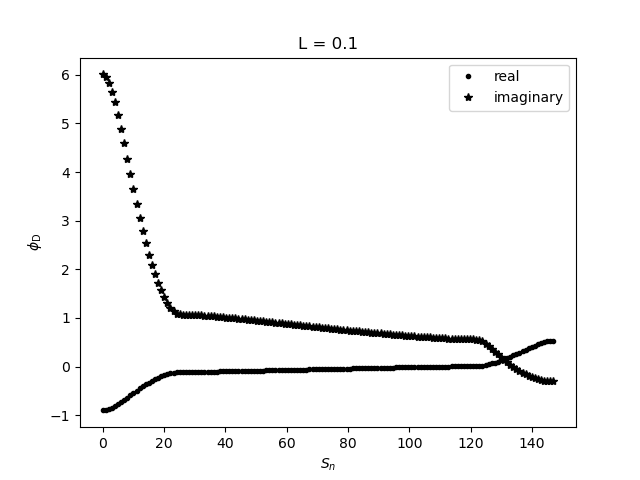
\includegraphics[width = \textwidth]{phiD_Lp1_kD1point2.png}
    \caption{$\phi_{\mathrm{D}}$ for $\sfrac{L}{D} = 0.1$.}
\end{Figure}
\begin{Figure}
    \centering
    \captionsetup{type = figure}
    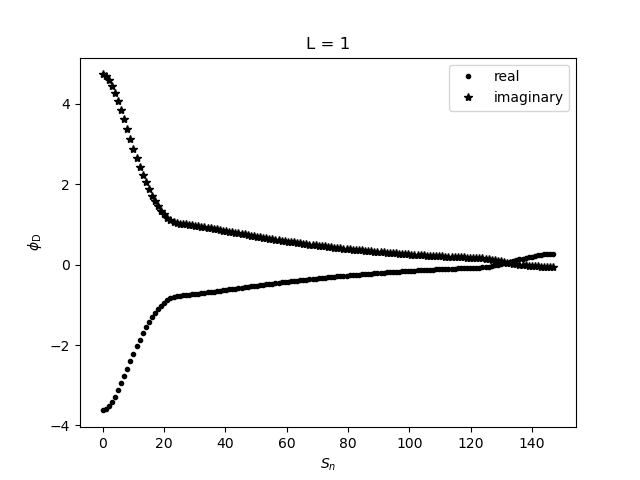
\includegraphics[width = \textwidth]{phiD_L1_kD1point2.png}
    \caption{$\phi_{\mathrm{D}}$ for $\sfrac{L}{D} = 1$.}
\end{Figure}
\begin{Figure}
    \centering
    \captionsetup{type = figure}
    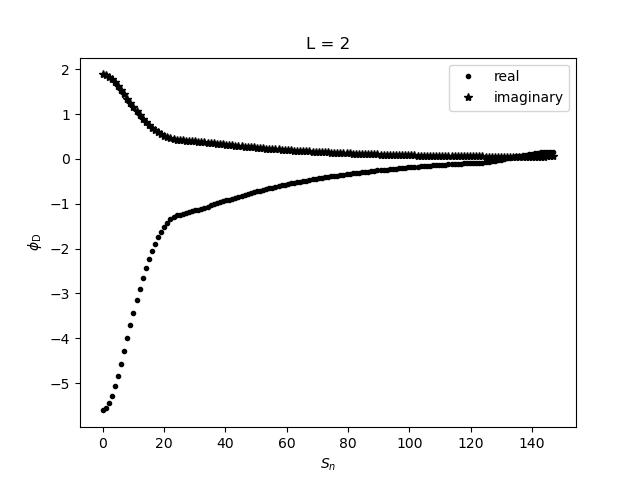
\includegraphics[width = \textwidth]{phiD_L2_kD1point2.png}
    \caption{$\phi_{\mathrm{D}}$ for $\sfrac{L}{D} = 2$.}
\end{Figure}
\begin{Figure}
    \centering
    \captionsetup{type = figure}
    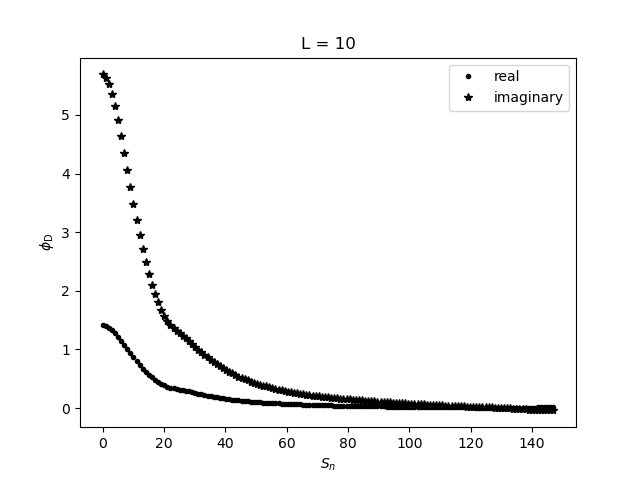
\includegraphics[width = \textwidth]{phiD_L10_kD1point2.png}
    \caption{$\phi_{\mathrm{D}}$ for $\sfrac{L}{D} = 10$.}
\end{Figure}
The exciting force may then be obtained through
\[
    X_2 = -i \omega \varrho \int_{S_{\mathrm{B}}} \phi_{\mathrm{D}} \hat{n}_2 \,\dee S.
\]
We also utilize the \textsc{Haskind} relations
\[
    X_{2}^{\mathrm{\textsc{h}}1} = -i \omega \varrho \int_{S_{\mathrm{B}}} \big( \phi_0 \partial_{\nhat} \phi_2 - \phi_2 \partial_{\nhat} \phi_0 \big) \,\dee S,
\]
\[
    X_{2}^{\mathrm{\textsc{h}}2} = i \varrho \gravity A_{2}^{-\infty},
\]
and the \textsc{Froude}--\textsc{Krylov} approximation
\[
    X_{2}^{\mathrm{\textsc{fk}}} = \varrho \gravity \sin{\left( \frac{\kappa L}{2} \right)} \frac{e^{-\kappa D}}{\kappa}.
\]
The \textsc{Haskind} relations and \textsc{Froude}--\textsc{Krylov} approximation will be derived in the lecture notes.
\begin{Figure}
    \centering
    \captionsetup{type = figure}
    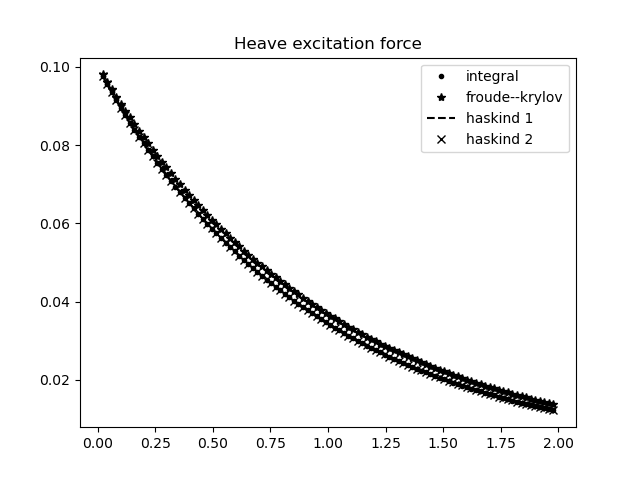
\includegraphics[width = \textwidth]{excitation_Lp1.png}
    \caption{Excitation force for $\sfrac{L}{D} = 0.1$.}
\end{Figure}
\begin{Figure}
    \centering
    \captionsetup{type = figure}
    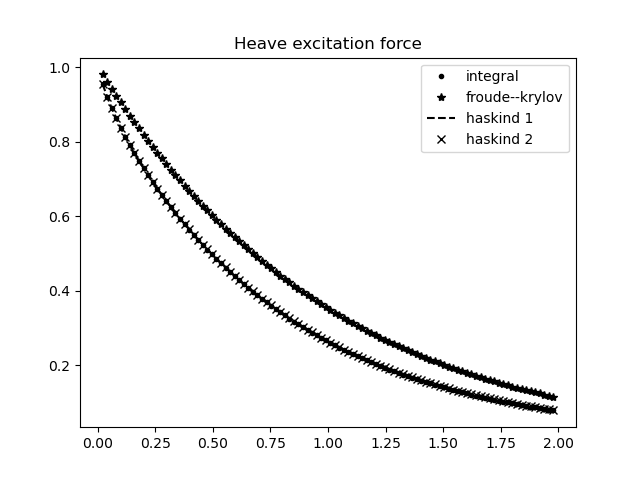
\includegraphics[width = \textwidth]{excitation_L1.png}
    \caption{Excitation force for $\sfrac{L}{D} = 1$.}
\end{Figure}
\begin{Figure}
    \centering
    \captionsetup{type = figure}
    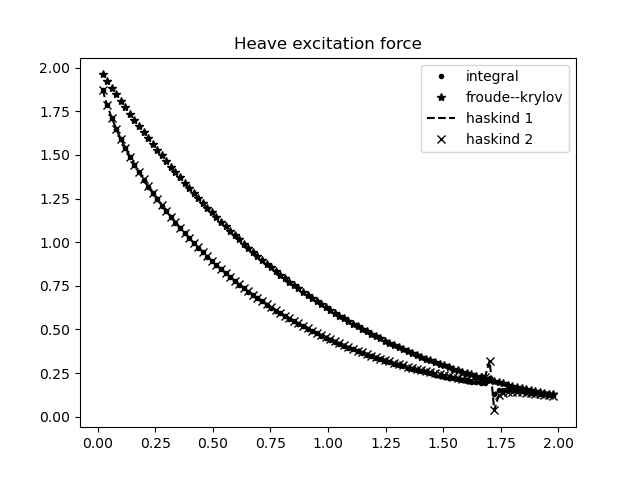
\includegraphics[width = \textwidth]{excitation_L2.png}
    \caption{Excitation force for $\sfrac{L}{D} = 2$.}
\end{Figure}
\begin{Figure}
    \centering
    \captionsetup{type = figure}
    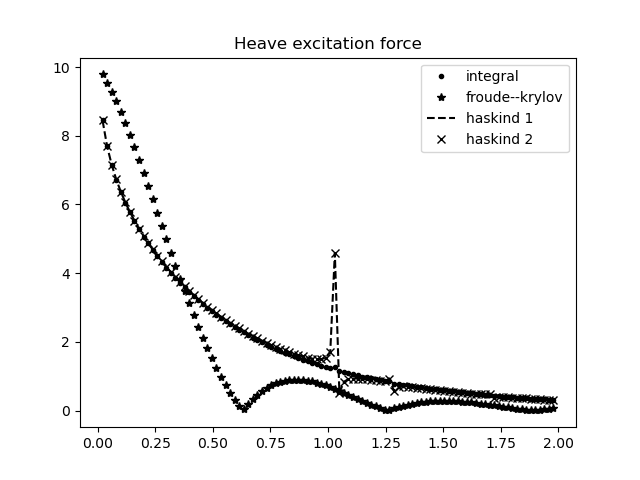
\includegraphics[width = \textwidth]{excitation_L10.png}
    \caption{Excitation force for $\sfrac{L}{D} = 10$.}
\end{Figure}
